\documentclass[letterpaper,11pt]{article}

\usepackage{spverbatim}
\usepackage{minted}
\usepackage{amssymb}
\usepackage{bm}
\usepackage{graphicx}
\usepackage{amsmath}

\usepackage{minted}
\usepackage{titling}
\newcommand{\subtitle}[1]{%
  \posttitle{%
    \par\end{center}
    \begin{center}\LARGE#1\end{center}
    \vskip0.5em}%
}

\usepackage{tabularx} % extra features for tabular environment
\usepackage{amsmath}  % improve math presentation
\usepackage{graphicx} % takes care of graphic including machinery
\usepackage[margin=1in,letterpaper]{geometry} % decreases margins
\usepackage{cite} % takes care of citations
\usepackage[final]{hyperref} % adds hyper links inside the generated
% pdf file
\usepackage{subcaption}
\usepackage{placeins}
%% \usepackage{placeins}

%% \hypersetup{
%% 	colorlinks=true,       % false: boxed links; true: colored links
%% 	linkcolor=blue,        % color of internal links
%% 	citecolor=blue,        % color of links to bibliography
%% 	filecolor=magenta,     % color of file links
%% 	urlcolor=blue
%% }
%++++++++++++++++++++++++++++++++++++++++

\title{\textbf{EECE 5639, Extra Credit Project:
\\{\Large Stereo}}}
\author{Sreejith Sreekumar}
\date{\today}

\begin{document}

\maketitle

\begin{abstract}
  In traditional stereo vision, two cameras, displaced horizontally from one another are used to obtain two differing views on a scene. By comparing these two images, the relative depth information can be obtained in the form of a disparity map, which encodes the difference in horizontal coordinates of corresponding image points. The values in this disparity map are inversely proportional to the scene depth at the corresponding pixel location. Building on these ideas we try to estimate the depth of a scene.
 \end{abstract}


\section{Description of Algorithms/ Concepts Involved}
In this section we list and describe all of the algorithms implemented in the completion of this
project.

\subsection{Corner Detection}
Harris Corner Detector is a corner detection operator that is commonly used in computer vision algorithms to extract corners and infer features of an image. This algorithm takes the differential of the corner score into account with reference to direction directly. The main equations in corner detection are given by:

\begin{itemize}
\item  Computation of M from gradient components
\[
  M = \sum\limits_{x,y} w(x,y)
    \begin{bmatrix}
      I_{x}^{2} & I_{x}I_{y} \\
      I_{x}I_{y} & I_{y} ^{2}
    \end{bmatrix}
\]
\item Intensity change in shifting window eigenvalue analysis:
\[
E(u, v) =
    \begin{bmatrix}
      u & v \\
    \end{bmatrix}
    \]
\item Corner Response Measure

\[
 R = det M - k\ trace^{2}(M)
\]

\item Threshold R to determine the corners.

\end{itemize}


\subsection{Non-Max Suppression}
The output of harris corner detection could be thought of as a heat
map, with a region of high magnitudes around a single corner. In order
to produce corners from this map, we define the local maxima within a
region as a corner, if it is above a certain threshold. To find these
local maxima we slide a 3x3 window over the image. Every pixel in the
window that is less then than maximum value in the window is set to
zero.

\subsection{Normalized Cross Correlation}
We use the corners as features to find the interesting points in each
image and determine pair-wise point correspondences. One of the
methods to compare these interesting regions is Normalized Cross Correlation. \\

Normalized Cross Correlation is defined by the equation:
\[
N_{fg}  = \sum\limits_{x,y} \hat{f}(i,j)\hat{g}(i,j)
\]
where
\[
  \hat{f} = \frac{f}{||f||} = \frac{f}{\sqrt{\Sigma_{[i,j] \in R} f^{2}(i,j)}}
  \]

\[
  \hat{g} = \frac{g}{||g||} = \frac{g}{\sqrt{\Sigma_{[i,j] \in R} g^{2}(i,j)}}
  \]
  In practice, we perform a brute force search between all possible
  combinations of points from both images. We then sort the results of
  this search by magnitude of correlation value. The N correspondences
  with the highest normalized correlation values are maintained. The
  resulting correspondences are then further pruned by realistic
  geometric constraints. In our case, we know the images represent a
  small lateral rotation. Correspondences with vertical translations
  greater than a small threshold, or lateral translations greater than
  a large threshold are said to not fit this constraint, and are
  deleted. The result is approximately 60 robust correspondences
  between the two images.

  \subsection{Stereo Vision and Epipolar Geometry}
  Stereo vision involves the vision dynamics involved when two cameras take pictures of the same scene, but they are separated by a distance. The shifted amount is called the disparity. The disparity at which objects in the image best match is used by the computer to calculate their depth information.\\
  Epipolar geometry is the geometry describing stero vision. The essential matrix is a 3 x 3 marix that
  encodes the epipolar geometry of the two views. Given a point in an image, multiplying by the Essential Matrix, will tell us the epipolar line in the second image where the corresponding point must be.\\
  
  
  \subsection{Fundemental Matrix}
  The fundamental matrix is a 3 x 3 matrix which relates corresponding points in stereo images. In epipolar geometry
  with homogeneous image coordinates, x and x' of corresponding points in a stereo image pair, F * x describes a line
  on which the corresponding point x' must line (epipolar line). \\
  The equation relating x, x' and F can be written as
\[
  x'^{T} F x = 0
  \]

  
\subsection{Disparity and Depth}
Disparity refers to the difference in image location of an object seen by the left and right camera images. The disparity of features between two stereo images are usually computed as a shift to the left of an image feature when viewed in the right image. Stereo images may not always be correctly aligned to allow for quick disparity calculation. For example, the set of cameras may be slightly rotated off level. Through a process known as image rectification, both images are rotated to allow for disparities in only the horizontal direction.\\
 Disparity information can be useful in depth/distance calculation. Disparity and distance from the cameras are inversely related. As the distance from the cameras increases, the disparity decreases. This allows for depth perception in stereo images. \\
  

\section{Experiments}
This section describes the intermediate steps and experiments
performed in the completion of this project.

\subsection{Reading the image inputs}

The input for the depth map computation are two images of a toy castle. The images are read and converted into grayscale for processing. For detecting the corner features, we add a padding of 20 pixels around the image around its borders. \\ 


\subsection{Detecting Corners in the Images}
Harris corner detection algorithm is applied on the images followed by a non max
supression and thresholding to get the co-ordinates of the corners
from the images. \\

Iterating through the corners detected for each image, we create
cropped neighborhoods for every corner with it at the center.
This way, we'd have N template patches corresponding to the N points
in the image which were detected to be corners. \\

Following this procedure, we do \textit{normalized cross correlation}
(subsection 1.3) on every template from the first image with every
other template of the second image, constituting a brute force search
of all point neighborhood correlation combinations between the
images. The results of this search are sorted by cross correlation
magnitude and all matches above a tuned correlation threshold are
kept. \\

The correspondences which were found hence are visualized below using lines of different
colors.

\begin{figure}[h]
  \centering
  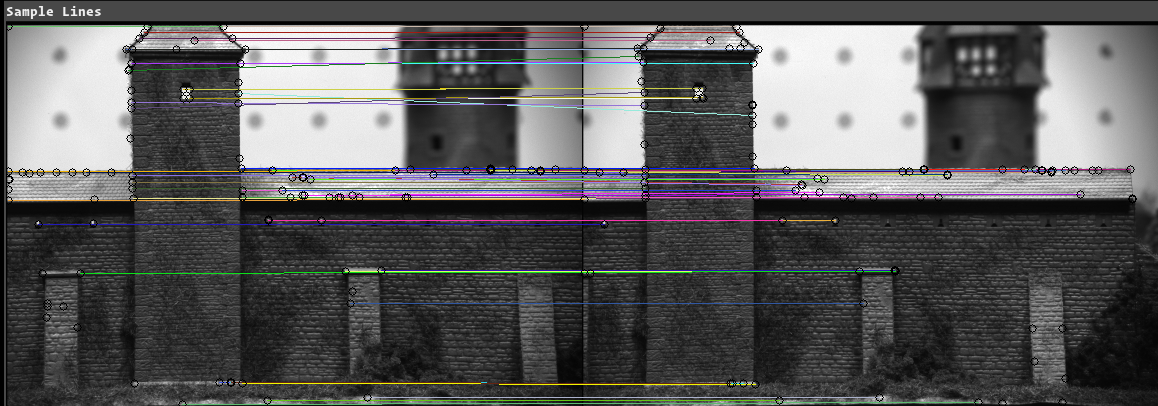
\includegraphics[width=\linewidth]{images/correspondences.png}
  \caption{Color Coded Corner Correspondences}
  \label{fig:sfig1}
\end{figure}

\subsection{Computation of Fundamental Matrix - 8 point algorithm}

The fundamental matrix is constructed from the mapped points using the 8 point algorithm.
The corresponding coordinates of every mapping is taken and we construct a matrix, \textit{A}
as: \\

\[
A = \begin{bmatrix} x_{1}x_{1}^{'} & x_{1}y_{1}^{'} & x_{1} & y_{1}x_{1}' & y_{1}y_{1}' & y_{1} & x_{1}' & y_{1}'& 1  \\ \vdots & \vdots & \vdots &\vdots &\vdots & \vdots & \vdots & \vdots &\vdots\\ x_{m}x_{m}^{'} & x_{m}y_{m}^{'} & x_{m} & y_{m}x_{m}' & y_{m}y_{m}' & y_{m} & x_{m}' & y_{m}'& 1 \end{bmatrix}
\]

Now we find the SVD of A, written by:
\[
A = UDV^{T}
\]

The columns of V are the eigenvectors of $A^{T}A$; the last one corresponds to the smallest eigenvalue. The entries of F are the components of the last column of V corresponding to the least singular value.

\subsection{Computing the disparity maps}

Now, using the properties of the fundamental matrix, for every point in the left image we compute the location of the corresponding point in the second image. The equation that relates the fundamental matrix and the co-ordinates can be given by:

\[
(F_{11}u_{1} + F_{12}v_{1} + F_{13})u + (F_{21}u_{1} + F_{22}v_{1} + F_{23})v + (F_{31}u_{1} + F_{32}v_{1} + F_{33}) = 0
\]

where $\begin{bmatrix} u \\ v \\ 1 \end{bmatrix}$ are the coordinates of the left image and $\begin{bmatrix} u_{1} \\ v_{1} \\ 1 \end{bmatrix}$ are the corresponding co-ordinates of the right image. \\
Hence for every co-ordinate in the right image we obtain the co-efficients of the equation of a line in the left image. \\

Setting the value of x to range from 0 to the width of the image, we compute the corresponding value of y, from the values of a, b and c (the co-ordinates of the line) as (-c-(a * x))/b. Those co-ordinates which fall within the limits of the image boundary of the left image are taken into consideration for finding the best corresponding point. For every point in the set of points we found hence, a patch around it is created, and correlation is computed. The co-ordinates around which the coorelation is maximum is taken as the corresponding left image point. \\

This procedure is repeated for every point in the right image to compute it's correspondence in the left image. \\

Once the correspondances have been figured out, the distance between the Xs and Ys of correspoinding pixels are computed. These values are taken as dispartity in the X direction and disparity in the Y direction repectively. Once the disparities have been computed, the depth is computed as the inverse of this measure. The disparity vector is computed as the magnitude of disparity vectors along the X and Y components at every pixel. The images hence generated are shown below. \\


\FloatBarrier
\begin{figure}[h]
\begin{subfigure}{.3\textwidth}
  \centering
  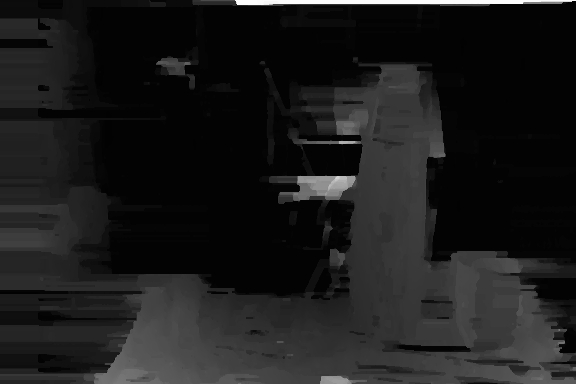
\includegraphics[width=.9\linewidth]{images/depthX.jpg}
  \caption{Vertical Disparity}
  \label{fig:sfig1}
\end{subfigure}%
\begin{subfigure}{.3\textwidth}
  \centering
  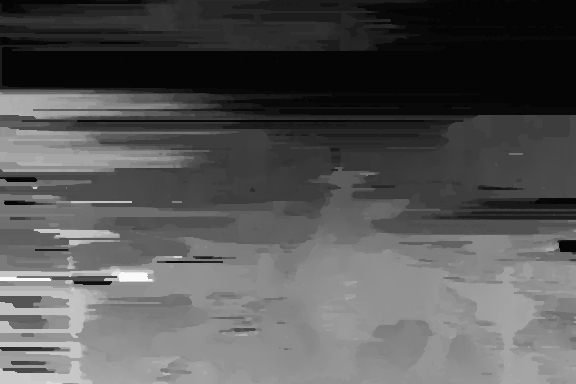
\includegraphics[width=.9\linewidth]{images/depthY.jpg}
  \caption{Horizontal Disparity}
  \label{fig:sfig1}
\end{subfigure}%
\begin{subfigure}{.3\textwidth}
  \centering
  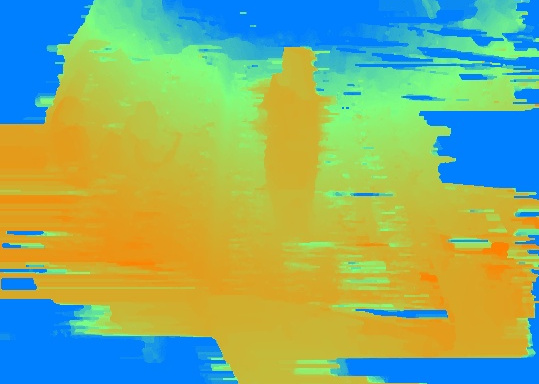
\includegraphics[width=.9\linewidth]{images/magnitude1.jpg}
  \caption{Disparity Vector}
  \label{fig:sfig2}
\end{subfigure}
\end{figure}


\section{Conclusion}
The two images were read in grayscale and corners in both of them were computed. We find the corner
correspondences using Harris corner detection. The corner correspondences were used in computing the
Fundamental matrix between the stereo images. The Fundemental matrix was used in finding the
pixel correspondences and the disparities were estimated. The disparity vector for every pixel was computed
and the same in both directions and the combined vector were represented as images.

\section{Appendix}

\subsection{Code}

\subsubsection{preprocess.cc}
\begin{minted}{C++}
#include <stdio.h>
#include <opencv2/opencv.hpp>
#include <opencv2/imgproc/imgproc.hpp>
#include <dirent.h>
#include <string>

using namespace cv;

std::vector<std::string> get_files(const char* path){

  /**
   *  Get all the image files from a path
   */

  DIR *dir;
  struct dirent *ent;

  std::vector<std::string> images;

  std::string dirname = path;
  if ((dir = opendir (path)) != NULL) {
    while ((ent = readdir (dir)) != NULL) {
      std::string file_name = ent->d_name;
      std::string full_path = dirname + "/" + file_name;

      images.push_back(full_path);
    }
    closedir (dir);
  } else {
    perror ("");
  }
  return images;
}


cv::Mat convertToGrayscale(cv::Mat color_image) {

  /**
   * Convert image to grayscale
   */
    cv::Mat greyMat;
    cv::cvtColor(color_image, greyMat, cv::COLOR_BGR2GRAY);
    return greyMat;

}

std::vector<cv::Mat> convertAllToGrayscale(std::vector<cv::Mat> color_images) {

    /**
     * Convert images to grayscale
     */
    std::vector<cv::Mat> gray_images;
    for (auto image = color_images.begin(); image != color_images.end(); ++image){
        cv::Mat gray;
        cv::cvtColor(*image, gray, cv::COLOR_BGR2GRAY);
        gray.convertTo(gray, CV_8U);
        //gray.convertTo(gray, CV_32S);
        gray_images.push_back(gray);
    }
    return gray_images;

}


std::vector<cv::Mat> addPadding(std::vector<cv::Mat> gray_images) {

    std::vector<cv::Mat> padded_images;
    for (auto image = gray_images.begin(); image != gray_images.end(); ++image){
      Mat padded;
      int pad = 20;
      copyMakeBorder(*image, *image, pad, pad, pad, pad, BORDER_CONSTANT);
      padded_images.push_back(*image);

    }
    return padded_images;
}


// std::vector<cv::Mat> addPadding2(std::vector<cv::Mat> gray_images) {

//     std::vector<cv::Mat> padded_images;
//     for (auto image = gray_images.begin(); image != gray_images.end(); ++image){
//       Mat padded;
//       int pad = 10;
//       copyMakeBorder(*image, *image, pad, pad, pad, pad, BORDER_CONSTANT);
//       padded_images.push_back(*image);

//     }
//     return padded_images;
// }


std::vector<cv::Mat> get_grayscale_images(std::vector<std::string> filenames){

  /**
   * Read the files as grayscale images and return
   * a vector of grayscale matrices that represents them
   *
   */
  std::vector<cv::Mat> grayimages;
  cv::Mat image;

  for(auto file = filenames.begin(); file != filenames.end(); ++file) {
    image = imread(*file);
    if ( image.empty() ){
      continue;
    }

    cv::Mat grayImage = convertToGrayscale(image);
    cv::Mat convertedGrayImage;
    grayImage.convertTo(convertedGrayImage, CV_8U);
    grayimages.push_back(convertedGrayImage);
  }

  return grayimages;

}

std::vector<cv::Mat> get_color_images(std::vector<std::string> filenames,
				      int scaleX, int scaleY){

  /**
   *Read RGB images and store in vector
   *
   */
    std::vector<cv::Mat> colorimages;
    cv::Mat image;

    for(auto file = filenames.begin(); file != filenames.end(); ++file) {
        image = imread(*file);
        if ( image.empty() ){
            continue;
        }
	cv::resize(image, image, cv::Size(), scaleX, scaleY);
        colorimages.push_back(image);
    }

    return colorimages;

}
\end{minted}

\subsubsection{utils.cc}

\begin{minted}{C++}
#include <iostream>
#include <opencv2/opencv.hpp>
#include <opencv2/highgui.hpp>

cv::Mat constructPointsMatrix(std::vector<PatchPair> mappings){


  /**
   *  Constrcut the m * 9 matrix A
   *
   */
  std::vector<std::vector<float>> _A;
    
  for(int i=0; i<mappings.size(); i++){


    std::vector<float> row;

    PatchPair pair = mappings[i];

    int x1 = pair.coordinate1[0];
    int y1 = pair.coordinate1[1];

    int x1_prime = pair.coordinate2[0];
    int y1_prime = pair.coordinate2[1];

    row.push_back(x1 * x1_prime);
    row.push_back(x1 * y1_prime);
    row.push_back(x1);
    row.push_back(y1 * x1_prime);
    row.push_back(y1 * y1_prime);
    row.push_back(y1);
    row.push_back(x1_prime);
    row.push_back(y1_prime);
    row.push_back(1);

    _A.push_back(row);
  }


  cv::Mat A(_A.size(), _A.at(0).size(), CV_32FC1);

  for(int i=0; i< A.rows; i++){
    for(int j=0; j< A.cols; j++){
       A.at<float>(i, j) = _A[i][j];
    }
  }


  return A;
  
  
}


std::vector<cv::Point> getCorrespondancePointsFromImage(std::vector<PatchPair> mappings,
							   int imageIndex){

  std::vector<cv::Point> points1;
  cv::Point2f point;
  
  for(int i=0; i<mappings.size(); i++){

      PatchPair pair = mappings[i];

      int x, y;

      if (imageIndex == 1){
	x = pair.coordinate1[0];
	y = pair.coordinate1[1];
      } else{
	x = pair.coordinate2[0];
	y = pair.coordinate2[1];
      }

      cv::Point point(x, y);

      points1.push_back(point);
      
 }

  return points1;
  
}



cv::Mat get_fundemental_matrix_after_ransac(std::vector<PatchPair> mappings){

  int point_count = mappings.size();

  vector<Point2f> points1(point_count);
  vector<Point2f> points2(point_count);

  for( int i = 0; i < point_count; i++ ){

    PatchPair pair = mappings[i];    

    int x1 = pair.coordinate1[0];
    int y1 = pair.coordinate1[1];

    int x1_prime = pair.coordinate2[0];
    int y1_prime = pair.coordinate2[1];    

    cv::Point2f pt1(x1, y1);
    cv::Point2f pt2(x1_prime, y1_prime);

    points1.push_back(pt1);
    points2.push_back(pt2);

  }

  cv::Mat fundamental_matrix = findFundamentalMat(points1, points2, FM_RANSAC);
  return fundamental_matrix;
    

}
\end{minted}

\subsubsection{visualization.cc}

\begin{minted}{C++}
# include <opencv2/opencv.hpp>
#include "opencv2/highgui/highgui.hpp"
#include "opencv2/imgproc/imgproc.hpp"
#include <stdio.h>
#include <stdlib.h>

using namespace cv;
using namespace std;


void imageCorrespondences(Mat im1,
			  Mat im2,
			  std::vector<PatchPair> mappings,
			  std::vector<std::vector<std::tuple<int, int, int>>> corners){

  // Test visualize correspondences
  Mat combined;
  Mat foo;
  hconcat(im1, im2, combined);
  cvtColor(combined, foo, COLOR_GRAY2BGR);   


  // Draw Lines
  for (int t = 0; t<mappings.size(); ++t){
    int r1 = mappings[t].coordinate1[0];
    int c1 = mappings[t].coordinate1[1];
    int r2 = mappings[t].coordinate2[0];
    int c2 = mappings[t].coordinate2[1];

    int r = 0 + ( std::rand() % ( 255 - 0 + 1 ) );
    int g = 0 + ( std::rand() % ( 255 - 0 + 1 ) );
    int b = 0 + ( std::rand() % ( 255 - 0 + 1 ) );    


    line(foo, Point(c1, r1), Point(c2+im1.cols, r2), CV_RGB(r, g, b), 1, 8);    
  }

  // Draw Corners on Image 1
  for (int t = 0; t < corners[0].size(); ++t){
    int r = get<1>(corners[0][t]);
    int c = get<2>(corners[0][t]);
    circle(foo, Point(c,r), 4.0, Scalar(0), 1, 8);    
  }

  // Draw Corners on Image 2
  for (int t = 0; t < corners[1].size(); ++t){
    int r = get<1>(corners[1][t]);
    int c = get<2>(corners[1][t]) + im1.cols;
    circle(foo, Point(c,r), 4.0, Scalar(0), 1, 8);    
  }

  // Display test frame
  namedWindow( "Sample Lines", WINDOW_AUTOSIZE );
  Mat sampleLines = foo;
  imshow("Sample Lines", foo);
  waitKey(0);

}
\end{minted}  

\subsubsection{epilines.cc}

\begin{minted}{C++}
#include <opencv2/core/core.hpp>
#include <opencv2/highgui/highgui.hpp>
#include <opencv2/calib3d/calib3d.hpp>
#include <opencv2/imgproc/imgproc.hpp>
/**
 * \brief Compute and draw the epipolar lines in two images
 *      associated to each other by a fundamental matrix
 *
 * \param title     Title of the window to display
 * \param F         Fundamental matrix
 * \param img1      First image
 * \param img2      Second image
 * \param points1   Set of points in the first image
 * \param points2   Set of points in the second image matching to the first set
 * \param inlierDistance      Points with a high distance to the epipolar lines are
 *                not displayed. If it is negative, all points are displayed
 **/
template <typename T1, typename T2>
static void drawEpipolarLines(const std::string& title, const cv::Matx<T1,3,3> F,
                const cv::Mat& img1, const cv::Mat& img2,
                const std::vector<cv::Point_<T2>> points1,
                const std::vector<cv::Point_<T2>> points2,
                const float inlierDistance = -1)
{
  CV_Assert(img1.size() == img2.size() && img1.type() == img2.type());
  cv::Mat outImg(img1.rows, img1.cols*2, CV_8UC3);
  cv::Rect rect1(0,0, img1.cols, img1.rows);
  cv::Rect rect2(img1.cols, 0, img1.cols, img1.rows);
  /*
   * Allow color drawing
   */
  if (img1.type() == CV_8U)
  {
    cv::cvtColor(img1, outImg(rect1), COLOR_GRAY2BGR);
    cv::cvtColor(img2, outImg(rect2), COLOR_GRAY2BGR);
  }
  else
  {
    img1.copyTo(outImg(rect1));
    img2.copyTo(outImg(rect2));
  }
  std::vector<cv::Vec<T2,3>> epilines1, epilines2;
  cv::computeCorrespondEpilines(points1, 1, F, epilines1); //Index starts with 1
  cv::computeCorrespondEpilines(points2, 2, F, epilines2);
 
  CV_Assert(points1.size() == points2.size() &&
        points2.size() == epilines1.size() &&
        epilines1.size() == epilines2.size());
 
  cv::RNG rng(0);
  for(size_t i=0; i<points1.size(); i++)
  {
    if(inlierDistance > 0)
    {
      if(distancePointLine(points1[i], epilines2[i]) > inlierDistance ||
        distancePointLine(points2[i], epilines1[i]) > inlierDistance)
      {
        //The point match is no inlier
        continue;
      }
    }
    /*
     * Epipolar lines of the 1st point set are drawn in the 2nd image and vice-versa
     */
    cv::Scalar color(rng(256),rng(256),rng(256));
 
    cv::line(outImg(rect2),
      cv::Point(0,-epilines1[i][2]/epilines1[i][1]),
      cv::Point(img1.cols,-(epilines1[i][2]+epilines1[i][0]*img1.cols)/epilines1[i][1]),
      color);
    cv::circle(outImg(rect1), points1[i], 3, color, -1, LINE_AA);
 
    cv::line(outImg(rect1),
      cv::Point(0,-epilines2[i][2]/epilines2[i][1]),
      cv::Point(img2.cols,-(epilines2[i][2]+epilines2[i][0]*img2.cols)/epilines2[i][1]),
      color);
    cv::circle(outImg(rect2), points2[i], 3, color, -1, LINE_AA);
  }
  cv::imshow(title, outImg);
  cv::waitKey(1);
}
 
template <typename T>
static float distancePointLine(const cv::Point_<T> point, const cv::Vec<T,3>& line)
{
  //Line is given as a*x + b*y + c = 0
  return fabsf(line(0)*point.x + line(1)*point.y + line(2))
      / std::sqrt(line(0)*line(0)+line(1)*line(1));
}
\end{minted}

\subsubsection{StereoUtils.cc}

\begin{minted}{C++}
#include <iostream>
#include <cmath>
#include <opencv2/opencv.hpp>
#include <opencv2/highgui.hpp>
#include <opencv2/imgproc/imgproc.hpp>


using namespace cv;


std::vector<int> getMaxCorrespondenceFromLine(int rightX,
					      int rightY,
					      std::vector<std::vector<int>> leftPoints,
					      cv::Mat leftImage,
					      cv::Mat rightImage){

  int x = rightX - 9 + 20;
  int y = rightY - 9 + 20;

  cv::Rect patchRegion(x, y,5, 5);
  cv::Mat rightPatch  = rightImage(patchRegion);
  cv::Mat rightPatchNorm = normalize(rightPatch);

  std::vector<float> correlations;

  for(int pointIndex=0; pointIndex < leftPoints.size(); pointIndex++){

    int leftImgXTmp = leftPoints[pointIndex][0];
    int leftImgYTmp = leftPoints[pointIndex][1];

    int xPatchLeftBegin = leftImgXTmp - 9 + 20;
    int yPatchLeftBegin = leftImgYTmp - 9 + 20;

    cv::Rect patchRegion(xPatchLeftBegin, yPatchLeftBegin, 5, 5);
    cv::Mat leftPatch = leftImage(patchRegion);
    cv::Mat leftPatchNorm = normalize(leftPatch);
	  
    cv::Scalar _correlation = cv::sum(rightPatchNorm.mul(leftPatchNorm));
    float correlation = _correlation[0];
    correlations.push_back(correlation);
	
   }

  int maxIndex = std::distance(correlations.begin(),
  			       std::max_element(correlations.begin(),
  						correlations.end()));

  return leftPoints[0];
}


std::vector<int> getCorrespondingPoint(int x_right,
				       int y_right,
				       int height,
				       int width,
				       cv::Mat fundamentalMatrix,
				       cv::Mat leftImage,
				       cv::Mat rightImage){

  float f11 = fundamentalMatrix.at<float>(Point(0,0));
  float f12 = fundamentalMatrix.at<float>(Point(1,0));
  float f13 = fundamentalMatrix.at<float>(Point(2,0));

  float f21 = fundamentalMatrix.at<float>(Point(0,1));
  float f22 = fundamentalMatrix.at<float>(Point(1,1));
  float f23 = fundamentalMatrix.at<float>(Point(2,1));

  float f31 = fundamentalMatrix.at<float>(Point(0,2));
  float f32 = fundamentalMatrix.at<float>(Point(1,2));
  float f33 = fundamentalMatrix.at<float>(Point(2,2));    

  /**
   * Co-efficients of the line
   */
  double a = (f11 * x_right) + (f12 * y_right) + f13;
  double b = (f21 * x_right) + (f22 * y_right) + f23;
  double c = (f31 * x_right) + (f32 * y_right) + f33;

  /**
   * get two points on this line
   */
  double x_min = 0;

  std::vector<std::vector<int>> points;

  for(int colIndex=20; colIndex<width; colIndex++){

    std::vector<int> co_ordinates;
      
    int rowIndex = floor((-c - (a * colIndex))/b);

    if((rowIndex >=20)  && (rowIndex < height - 20)){
      co_ordinates.push_back(colIndex);
      co_ordinates.push_back(rowIndex);

      points.push_back(co_ordinates);
    }

  }

  std::vector<int> correspondingPoint;


  if(points.size()>0){
    correspondingPoint =
      getMaxCorrespondenceFromLine(x_right, y_right, points, leftImage, rightImage);
  }

  return correspondingPoint;
}


void getDisparityMap(cv::Mat leftImage,
		     cv::Mat rightImage,
		     cv::Mat fundamentalMatrix){


  int width = rightImage.cols;
  int height = rightImage.rows;


  cv::Mat dispX(width,height, CV_8U);
  cv::Mat dispY(width,height, CV_8U);
  cv::Mat dispVector(width,height, CV_8U);      

  cv::Mat disparityMapX(height, width, CV_32F);
  cv::Mat disparityMapY(height, width, CV_32F);    
  
  for(int i=0; i<height; i++){
    for(int j=0; j<width; j++){

      vector<int> point = getCorrespondingPoint(i,
      						j,
      						height,
      						width,
      						fundamentalMatrix,
      						leftImage,
      						rightImage);
      int leftX = i;
      int leftY = j;

      int rightX = 0;
      int rightY = 0;
	  
      if(point.size()>0){

      	rightX = point[0];
      	rightY = point[1];

      }

      int disparityX = abs(rightX - leftX);
      int disparityY = abs(rightY - leftY);

      disparityMapX.at<float>(i,j) = disparityX;
      disparityMapY.at<float>(i,j) = disparityY;      
      
    }

  }

  double minValX; 
  double maxValX; 
  Point minLocX; 
  Point maxLocX;

  minMaxLoc( disparityMapX, &minValX, &maxValX, &minLocX, &maxLocX);

  disparityMapX -= minValX;
  disparityMapX.convertTo(dispX,CV_8U,255.0/(maxValX-minValX));

  namedWindow( "Disparity Horizontal", WINDOW_AUTOSIZE );  
  imshow("Disparity Horizontal", dispX);
  waitKey(0);
  

  double minValY; 
  double maxValY; 
  Point minLocY; 
  Point maxLocY;

  minMaxLoc( disparityMapY, &minValY, &maxValY, &minLocY, &maxLocY);

  disparityMapY -= minValY;
  disparityMapY.convertTo(dispY,CV_8U,255.0/(maxValY-minValY));


  namedWindow( "Disparity Vertical", WINDOW_AUTOSIZE );  
  imshow("Disparity Vertical", dispY);
  waitKey(0);

  cv::magnitude(dispX, dispY, dispVector);
  namedWindow( "Disparity Vector", WINDOW_AUTOSIZE );  
  imshow("Disparity Vector", dispY);
  waitKey(0);

}
  
\end{minted}

\subsubsection{main.cc}

\begin{minted}{C++}
#include "Config.cc"
#include "Preprocess.cc"
#include "Corners.cc"
#include "Visualization.cc"
#include "Utils.cc"
#include "Epilines.cc"
#include "StereoUtils.cc"

#include <algorithm>
#include <random>

#include <iostream>
#include <opencv2/opencv.hpp>
#include <opencv2/highgui.hpp>



using namespace std;
using namespace cv;


int main(){


  std::map<std::string,std::string> config = loadConfig("./src/config.cfg");
  std::vector<std::string> image_filenames = get_files("./data/");
  std::sort(image_filenames.begin(), image_filenames.end());

  /**
   * (a-i) Reading and Scaling
   */
  std::vector<cv::Mat> color_images = get_color_images(image_filenames, 1 , 1);
  std::vector<cv::Mat> gray_images = convertAllToGrayscale(color_images);
  std::vector<cv::Mat> padded_images = addPadding(gray_images);


  /**
   * (a-ii) Sparse corner coordinates
   */

  int threshold = 60;
  int cornerCount = 100;

  std::vector<std::vector<std::tuple<int, int, int>>> corners = getCornersInImageArray(gray_images,
  										       threshold,
  										       cornerCount);

  std::vector<std::vector<Template>> patches = createPatches(padded_images,
  							     corners);
  std::vector<PatchPair> patch_correlations_sorted = comparePatches(patches[0],
  								    patches[1]);


  /**
   * (a-iii) Find corner correspondences
   */

  std::vector<PatchPair> mappings = removeDuplicateCorrespondences(patch_correlations_sorted);

  // Prune correspondences based on geometric constraints
  for (int i = mappings.size() - 1; i >= 0; i--){
    if (abs(mappings.at(i).coordinate1[0] - mappings.at(i).coordinate2[0]) > 30 ||
  	abs(mappings.at(i).coordinate1[1] - mappings.at(i).coordinate2[1]) > 250){
      mappings.erase( mappings.begin() + i );
    }
  }


  // castle left
  Mat im1 = gray_images[0];
  // castle right
  Mat im2 = gray_images[1];
  imageCorrespondences(im1, im2, mappings, corners);


  /**
   *   Calculation of the fundemental Matrix
   *   Construct the matrix 
   *
   */

  cv::Mat A = constructPointsMatrix(mappings);
  cv::Mat W, U, Vt;
  cv::SVD::compute(A, W, U, Vt)	;

  cv::Mat fundMat(3,3, CV_32F);

  fundMat.at<float>(0,0) = Vt.at<float>(0,8);
  fundMat.at<float>(0,1) = Vt.at<float>(1,8);
  fundMat.at<float>(0,2) = Vt.at<float>(2,8);
  fundMat.at<float>(1,0) = Vt.at<float>(3,8);
  fundMat.at<float>(1,1) = Vt.at<float>(4,8);
  fundMat.at<float>(1,2) = Vt.at<float>(5,8);
  fundMat.at<float>(2,0) = Vt.at<float>(6,8);
  fundMat.at<float>(2,1) = Vt.at<float>(7,8);
  fundMat.at<float>(2,2) = Vt.at<float>(8,8);

  // cv::Mat fundamentalMatrix = get_fundemental_matrix_after_ransac(mappings);
  // std::cout<<"Fundemental Matrix after RANSAC on correspoinding points \n "
  // 	   <<fundamentalMatrix<<"\n";


  /**
   *  dense Disparity Map
   */
   getDisparityMap(padded_images[0], padded_images[1], fundMat);
  

}
\end{minted}  


\end{document}
